\chapter{Theoretical Background}
\section{Single-particle dynamics in electron storage rings}
For the proper understanding of the experiments carried out during the reported period, a brief theoretical background section is provided.
\subsection{Motion of charged particles in magnetic fields}
An electron with charge $e$ and momentum $p$ follows a circular orbit of radius $\rho$ when under the influence of an uniform and constant magnetic field with magnitude $B$, perpendicular to the ortbit plane. In such conditions, Lorentz force law predicts that
\begin{equation}
    B\rho = \frac{p}{e}.
\end{equation}

For an electron traveling along a curve parametrized by the arclength $s$ and under the influence of fields $B_x(x,y,s)$  and $B_y(x,y,s)$, perpendicular to its direction of motion, the deflection angles in the transverse planes normal and bi-normal to the trajcetory are given by
    \begin{equation}
    \dd{\theta_x} = \frac{\dd{s}}{\rho_x(s)} = \frac{e}{p}B_y(x,y,s)\dd s = \frac{1}{B\rho}B_y(x,y,s)\dd s,
    \end{equation}
    \begin{equation}
        \dd{\theta_y} = \frac{\dd{s}}{\rho_y(s)} = \frac{e}{p}B_x(x,y,s)\dd s = \frac{1}{B\rho}B_y(x,y,s)\dd s.
    \end{equation}
Where eq. (1) has been used to replace the $p/e$ ratio by the \textit{magnetic rigity} $B\rho$, which is defined as the product of the uniform field strength needed for a beam with momentum $p$ and charge $e$ to perform circular orbit with radius $\rho$. The rigidity depends solely on the electron's momentum/energy and gives the appropriate normalization to evaluate the instantaneous angular deflections in the electron's trajectory caused by magnetic fields.
\subsection{Storage rings}
\begin{figure}[htb]
    \centering
    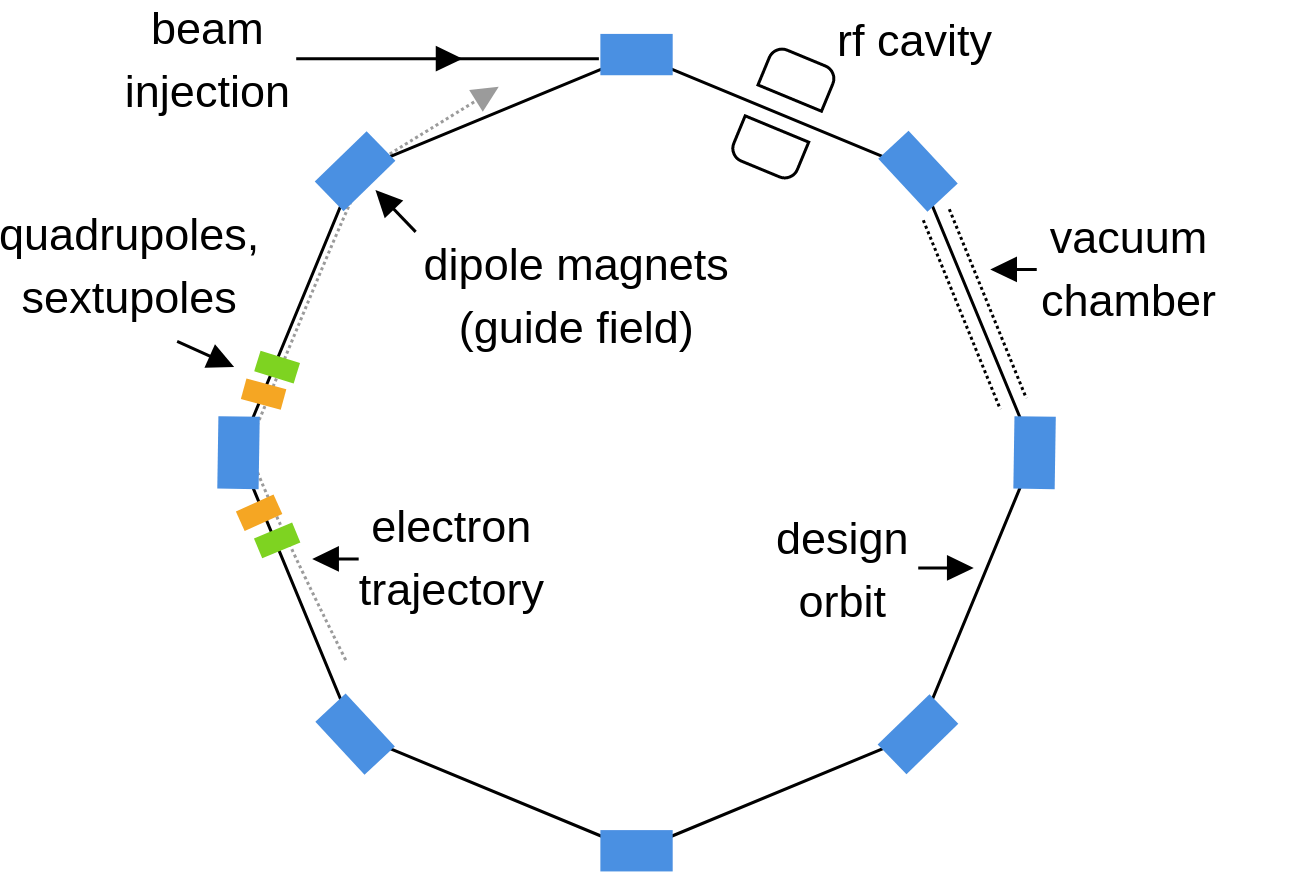
\includegraphics[width=0.4\textwidth]{Images/storage_ring.png}
    \caption{Storage ring typycal configuration. From \cite{sands}}
    \label{sr}
\end{figure}
Figure~\ref{sr} sketches the typical design of a storage ring. For the porpose of storing a beam of electrons in closed orbits, magnetic fields defining a closed orbit is necessary. The angular deflections should add up to $2\pi$, so the specification of the beam's operating energy will determine the integrated field required for such deflections. Magnets specifying the curvature radius and the reference orbit are sectionally uniform and provided by dipole magnets.

Focusing towards the reference closed orbit is also needed, and can be attained with the introduction of gradient field with strengths depending linearly with tranverse excursions from the reference orbit. Such fields are provided by quadrupole magnets, which are physically realized by specifying  magnetic poles with the shape of truncated hyperbolas.

Sextupole mangets are also usually included in the design of storage rings. The fields they produce is quadratic with transverse displacement and are needed for correction of chromatic errors in the dynamics.

\subsection{The coordinate system}
\begin{figure}[htb]
    \centering
    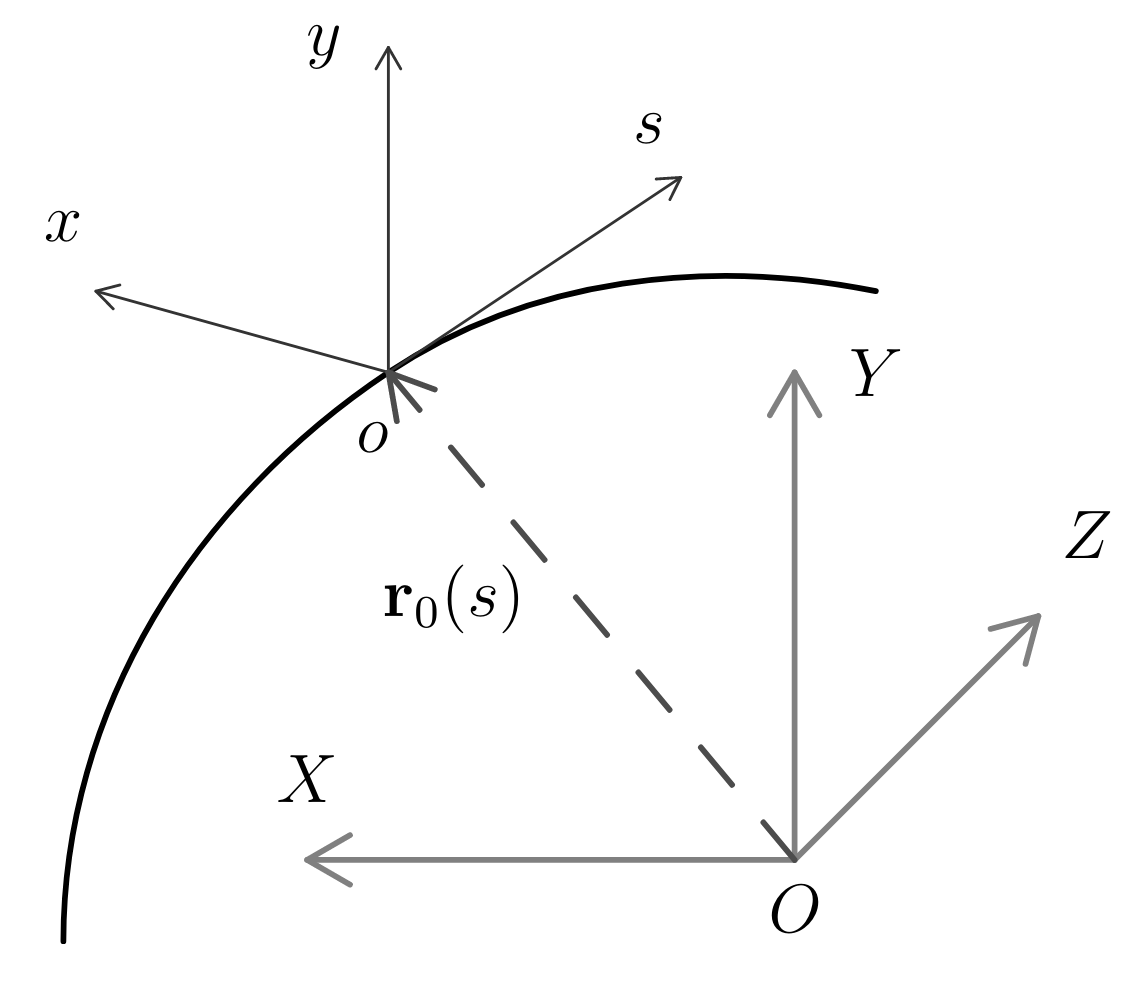
\includegraphics[width=0.6\textwidth]{Images/frenetserret.png}
    \caption{The Frenet-Serret coordinate system. From \cite{huang2019beam}.}
    \label{frenetserret}
\end{figure}
To conveniently decribe the dynamics in storge rings, our reference frame should be able to capture the deviations from the nonimal reference orbit and the beam design parameters. This can be attained by imagining a reference particle traveling along a curve drawn by the tip of the vector $\vb{r}_0$, as Fig.~\ref{frenetserret} shows. The particle travels a distance $s$ along the ring, which can be used to parametrize the motion. The reference frame triad of direction vectors consists of a vector $\vu{s}$, tangent to the trajectory, a vector $\vu{x}$ normal to it, pointing in the direction at which $\vu{s}$ changes and a vector $\vu{y}=\vu{x}\cross\vu{s}$, bi-normal to the trajectory. This construction leads to a Frenet-Serret reference frame.

Assuming no curvature in the $y$ plane, i.e. that the accelerator defines a curve whose plane is parallel to the ground, the Frent-Serret frame is defined by \cite{lee}
\begin{equation}
\vu{s}=\dv{\vb{r}_{0}}{s}, \quad \vu{x}=-\rho\dv{\vu{s}}{s}, \quad \vu{y} =  \vu{x}\times\vu{s},
\end{equation}
    and evolve along $s$ as prescribed by the Frenet-Serret equations:
\begin{equation}
\dv{\vu{s}}{s}=-\frac{1}{\rho(s)}\vu{x}, \quad\dv{\vu{x}}{s}=\frac{1}{\rho(s)}\vu{s}, \quad \dv{\vu{y}}{s}=0,
\end{equation}
where $\rho(s)$ is the local curvature radius. The frame thus depends solely on the geometry of the specified path. Since the curvature is defined by the magnetic lattice, if the storage ring is composed of dipole fields $B_0(s)$ in the $y$ direction, then, eq. (1) leads to
    \begin{equation}
        G(s) \equiv \frac{1}{\rho(s)} = \frac{B_0}{B\rho}.
        \label{G}
    \end{equation}

\subsection{Hamiltonian for the relativistic electron}
The dynamics of relativistic electrons influenced by electromagnetic fields $(\Phi, \vb{A})$ is encapsulated by the Hamiltonian
    \begin{equation*}
        H=\sqrt{m^2c^4+(\vb{P}-q\vb{A})^2c^2}+e\Phi,
    \end{equation*}
 $e$ being the elementary charge and $\vb{P}=\vb{p}+e\vb{A}$ the canonical momentum. The following steps are followed to obtain equations of motion for electrons in the storage ring:
 \begin{itemize}
    \item A canonical transformation to change coordinates is applied in order to describe the motion in terms of the Frenet-Serret frame variables;
    \item Instead of time $t$, the Hamiltonian and the dynamical variables are described as functions of $s$, the longitudinal position along the ring;
    \item Geometric quantities are used: canonical momenta are the angles with respect to the nominal orbit;
    \item Paraxial approximation: transverse momenta are assumed to be way smaller than longitudinal momentum
 \end{itemize}
 all of these steps are shown in detail in textbooks such as  Refs.~\cite{lee, wiedemann,  wolski2014beam}. For the purpose of examining the DA, we can model the motion withouth RF cavities ($\Phi=0$) and neglect radiation losses. The dynamics will consist solely on the transverse degrees of freedom, and takes place on a 4-dimensional phase space. In this 4D dynamics, the set of canonical variables are $(x,p_{x},y , p_{y})$, where
\begin{equation}\begin{cases} p_{x}= x^\prime(1+\delta),\\p_{y}=y^\prime (1+\delta),\end{cases}\end{equation}
and the energy/momentum deviation is an additional parameter
\begin{equation}
    \delta = \frac{P-P_{0}}{P_{0}}\approx\frac{E-E_0}{E_0}
\end{equation}
where the ultra-relativistic approximation $E\approx pc$ was used.

Hamilton's equations for the Hamiltonian in the paraxial approximation lead to the equations of motion for 4D dynamics
\begin{equation}
x^{\prime \prime}=-\frac{(1+G x)^{2}}{1+\delta} \frac{B_{y}}{B \rho}+G(1+G x),
\quad
y^{\prime \prime}=\frac{(1+G x)^{2}}{1+\delta} \frac{B_{x}}{B \rho}
\end{equation}
where $B\rho = p/e$ and $G(s)$ defined as in Eq.~\eqref{G}.
\subsubsection{The Magnetic Fields}
Fields influencing the beam are those of dipoles, quadrupoles and sextupoles.
Their functional forms are
\begin{itemize}
    \item Horizontal Dipole:\\
           $$ B_x = 0, \quad B_y = B_0$$
    \item Normal quadrupole\\
          $$B_x = B_1 y, \quad B_y = B_1 x$$
    \item Normal sextupole\\
          $$B_x = B_2xy, \quad B_y = \frac{1}{2}B_2(x^2 - y^2)$$
\end{itemize}
These are the so-called normal multipole fields. There also exists skew multipole fields, which couple the horizontal and vertical dynamics. We will neglect skew fields and coupling for now.

In the equations of motion, the magnetic rigidity normalizes all the fields. So we define the dipolar, quadrupolar and sextupolar functions by
$$G(s) = \frac{B_0(s)}{B\rho}, \quad K(s) = \frac{B_1(s)}{B\rho}, \quad S(s) = \frac{B_2(s)}{B\rho}$$

\subsection{Linear Dynamics}
\subsubsection{Linear equations of motion}
Expansion of the equations of motion up to first order in the $x, y, \delta$ variables leads to \cite{sands}
    \begin{equation}
        x^{\prime\prime}+(G^2+K)x=G\delta, \quad
        y^{\prime\prime}-Ky=0.
    \end{equation}
    For on-momentum particles, $\delta=0$, both equations reduce to Hill's equations
    \begin{equation}
        u^{\prime\prime}+K_u(s)u = 0,
    \end{equation}
    which are a pair of parametric oscillators for $u=x,y$, with $s$-dependent focusing functions
         $$K_x(s) = G^2(s) + K(s)$$ $$K_y(s) = - K(s)$$
Motion in the linear approximation thus consists on oscilations around the closed orbit, known as betatron oscillations.
\subsubsection{Pseudoharmonic description}
The solutions for the equations of betatron motion can be cast in a amplitude-phase (WKB) form
\begin{equation}
    u(s) = \sqrt{2\beta_u(s) J_u}\cos(\phi_u(s) + \phi_0),
\end{equation}
where $\beta_u(s)$ must satify the boundary value problem
\begin{equation}
    \frac{1}{2}\beta_{u}^{\prime\prime}+\beta_{u} K_u(s) - \frac{1}{\beta_{u}}\qty(\frac{1}{4}\beta_{u}^{\prime 2} + 1 ) = 0, \quad
        \begin{cases}
            \beta_{u}(0) = \beta_{u}(L)\\ \beta_{u}^{\prime}(0) = \beta_{u}^{\prime}(L)
        \end{cases}
\end{equation}
and the phase advance is
    \begin{equation}
        \phi_u(s) = \int_{0}^{s}\frac{1}{\beta_u(\sigma)}\dd\sigma.
   \end{equation}
The betatron functions for the SIRIUS storage ring are shown in Fig.~\ref{betafunc}.
\begin{figure}[htb]
    \centering
    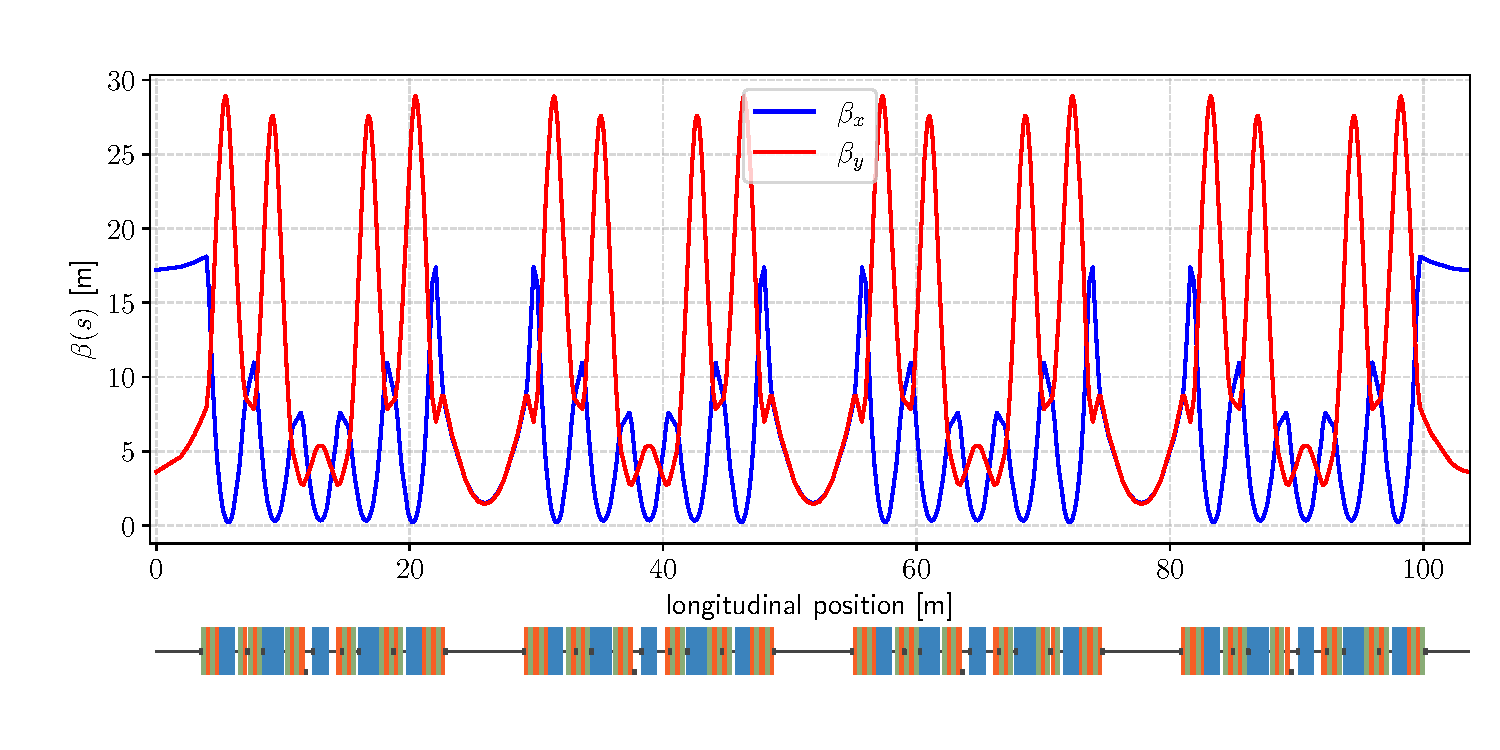
\includegraphics[width=\textwidth]{Images/beta_functions.pdf}
    \caption{Betatron functions for the SIRIUS storage ring. Colored blocks represent the magnets of the accelerator lattice: blue for dipoles, orange for quadrupoles and green for sextupoles. The ring has a 5-fold symmetry, with the lattice and betatron function repeating the same pattern shown above five times up to $s=518~\unit{m}$}
    \label{betafunc}
\end{figure}

An important feature of the dynamics is the \textit{tune}: the phase advance per ring revolution
\begin{equation*}
    \nu_u=\frac{1}{2\pi}\int_{s}^{s+L}\frac{\dd \sigma}{\beta_u(\sigma)}\equiv\frac{1}{2\pi}\oint\frac{\dd s}{\beta_u(s)}.
\end{equation*}
The analysis of perturbations and nonlinearities shows that the tunes are a critical variables in determining the beam's response to perturbations. More specifically, the tunes impact over disturbances amplifiction factors, which are greatest when tunes are close to integer numbers.

SIRIUS ring has tunes $(\nu_x, \nu_y)=(49.08, 14.14)$ which are very close to integers. It is desired to increase the tunes fractional parts to reduce orbit amplification factors. This is the reason why injection efficiency optimzation runs have also been carried in different machine tunes.
\subsubsection{Turn-by-turn data}
In the $u, u^\prime$ phase space, the quasi-periodic motion traces out ellipses. This can be verified by calculating the derivative $u^\prime$, defining $\alpha_u = \frac{\beta_u^\prime}{2}$  and $\gamma_u = \frac{(1+\alpha_u^2)}{\beta_u}$ and checking that $u, u^\prime$ satify the quadratic form
        $$2J_u=\gamma u^{2}+2\alpha u u^{\prime}+\beta u^{\prime2}$$
The ellipse properties are defined by the $\beta, \alpha$ and $\gamma$ functions, also known as Courant-Snyder Parameters or Twiss Parameters. These are functions of the position $s$, so at each point along the accelerator the Poincaré Section $u, u^\prime$ displays a different ellipse, with shape dictated by the Twiss parameters.
\begin{figure}[htb]
    \centering
    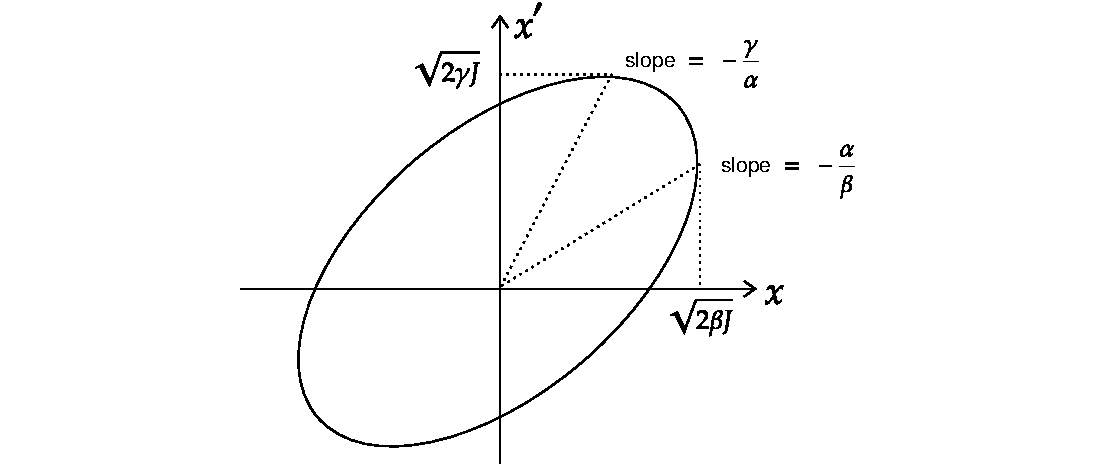
\includegraphics[width=0.5\textwidth]{Images/ellipse}
    \caption{Phase space ellipse traced by tur-by-turn (TbT) motion in the $(x,p_x)$ phase space. Optics functions determine the principal axes ratios and the inclination of the ellipse at each longitudinal position along the ring. From \cite{wolski2014beam}.}
    \label{ellipse}
\end{figure}
\subsection{Chromatic effects}
\subsubsection{Dispersion}
The equation of motion for off-momentum particles in the horizontal plane is the non-homogeneous Hill's equation. The solution consists on the linear combination of the homogeneous solutions in the phase-amplitude form plus the particular solution: $x=x_\beta+ x_\delta = x_\beta+ \eta(s)\delta $ where $\eta(s)$ is the \textit{dispersion function}, satisfying
    \begin{equation*}
        \eta^{\prime\prime}+(G^2+K)\eta=G,\quad
        \begin{cases}
            \eta(0) = \eta(L),\\
            \eta^\prime(0) = \eta^\prime(L).
        \end{cases}
    \end{equation*}
    The periodicity in the $\eta(s)$ function is required if we want to interpret $\eta$ as closed orbit per momentum deviation. Thus, off-momentum particles perform betatron oscillations around a dispersive orbit. The dispersion function for the SIRIUS storage ring is shown in Fig.~\ref{dispersion_func}
    \begin{figure}[htb]
        \centering
        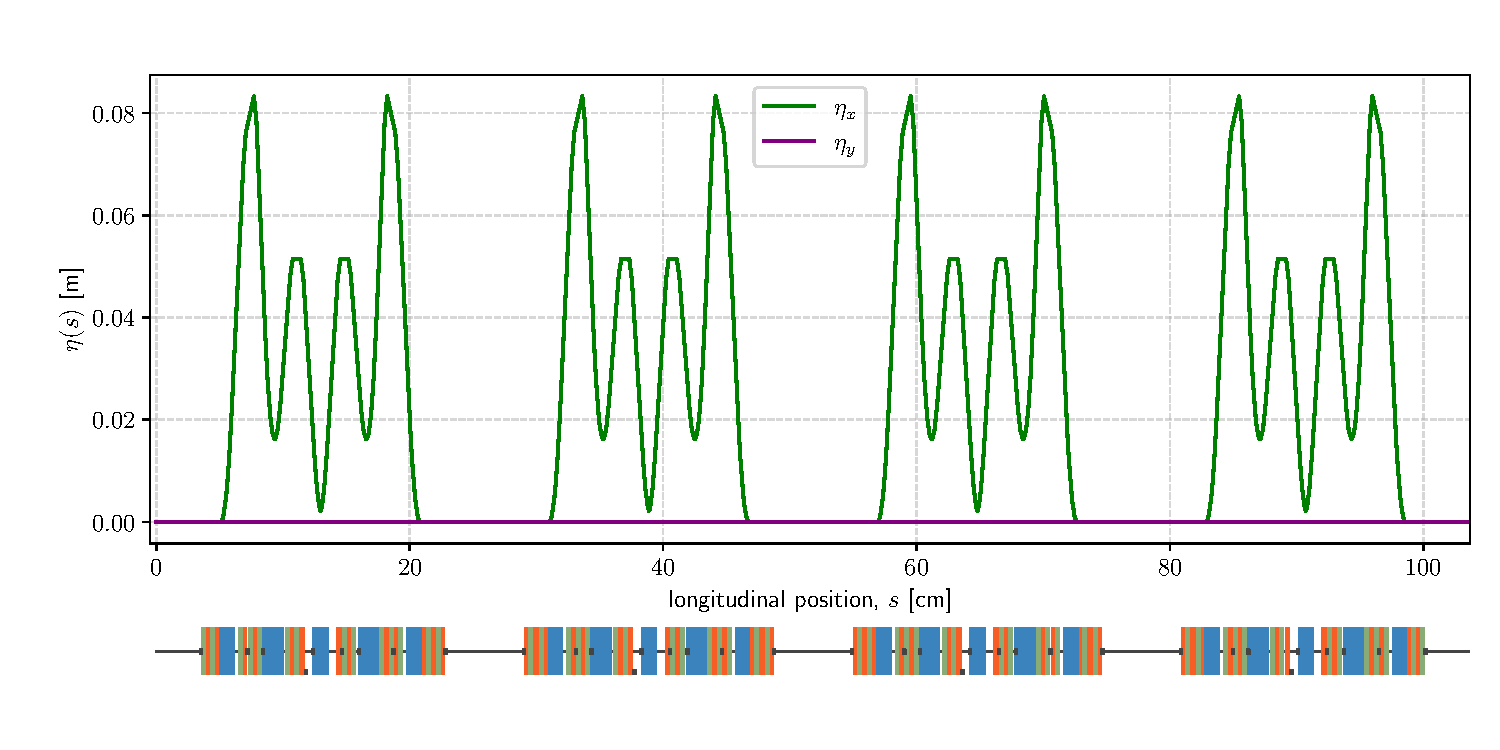
\includegraphics[width=\textwidth]{Images/dispersion.pdf}
        \caption{Dispersion fucntion for SIRIUS superperiod.}
        \label{dispersion_func}
    \end{figure}
\subsubsection{Chromaticity}
Energy deviations affect not only the closed orbit but also the focusing. A more/less energetic beam has higer/lower rigidity and thus is focused differently when passes through quadrupoles. This chromatic aberration effect needs to be currected, which can be attained with the insertion of geometric aberrations provided by sextupolar fields. The correction comes at the expense of introducing nonlinearities in the dynamics.

The focusing errors due to energy errors cause phase advance errors and consequently tune errors, or tune-shifts. As a first order approximation,
\begin{equation}
    \Delta \nu_u = \xi_u \delta,
\end{equation}
where the tune-shift per energy deviation $\xi_u$ is the chromaticity, which depends linearly on quadrupoles and sextupoles strengths. This linear dependence allows for the correction of chromaticity and control of the focusing for off-energy particles.
\subsection{Nonlinear Dynamics}
\subsubsection{Action Angle Variables}
Betatron motion (Hill's equations) can be obtained from the Hamiltonian
\begin{equation}
    \mathcal{H}=\frac{1}{2}u^{\prime2}+\frac{1}{2}K_u(s)u^2.
\end{equation}
The transformation $(u,u^\prime)\to(\psi, J)$ to Action-angle variables is implicitly implemented by the generating function
\begin{equation}
    F_1(u,\phi_u)=\int{u}^\prime\dd{{u}}=\frac{u^2}{2\beta_u}\qty(\tan \phi_u-\frac{\beta_u^\prime}{2}).
\end{equation}
The action variable reads
\begin{equation}
    J_u=-\pdv{F_1}{\phi_u} = \frac{u}{2\beta_u}\sec^2\phi_u = \frac{1}{2\beta_u}[u^2 + (\beta_u u^\prime + \alpha_u u^2)],
    \label{eq:action}
\end{equation}
and we recover the pseudo-harmonic form $u=\sqrt{2\beta J_u}\cos(\phi_u(s)+\phi_0)$, which has been conveniently defined so one of the constants to be detemined, $J_u$, corresponds to the action variable.

in the $J,\phi$ variables, the new hamiltonian is $H_0(\phi, J)$,  given by
\begin{equation}
    H_0=\mathcal{H}+\pdv{F_1}{s} = \frac{J}{\beta}.
\end{equation}
Performing the change to action-angle variable in both the horizontal and vertical planes we find the new Hamiltonian for 4D dynamics
\begin{equation}
    H_0= \frac{J_x}{\beta_x} +  \frac{J_y}{\beta_y},
\end{equation}
and Hamilton's equations are
\begin{equation}
    \phi_u^\prime = \frac{1}{\beta_u(s)},\qquad J_u^\prime=0.
\end{equation}
\subsubsection{Perturbations and tune-shifts}
Linear motion is integrable, since it can be written in terms of the action variable only (angle-independent Hamiltonian). This leads to the action variable being a constant of motion, and the phase advance behaving just as the pseudo-harmonic motion anticipated.

Linear motion, though, is only a useful first approximation. In reality, in an storage ring we have higher order multipole magnets, such as sextupole magnets, and also multipole, alignement and excitation errors, all acting as perturbations to linear motion. Generically refering to perturbations as $V(J, \phi)$, we have the perturbed motion Hamiltonian
\begin{equation}
    H(J,\phi) =H_0 + V(J,\phi),
\end{equation}
and hamilton's equations
\begin{equation}
\phi_u^\prime = \frac{1}{\beta_u(s)}+\pdv{V(J,\phi)}{J_u}, \quad J_u^\prime = \pdv{V(J,\phi)}{\phi_u}.
\end{equation}
Since the tunes consist on the phase advance per revolution, we immediately see that the presence of perturbations lead to tune-shifts. Generically, the tunes can be expressed in terms of the tune-shifts as
$$\nu_0 = \nu_{u0} + \xi_u(\delta) \delta + \alpha_{uu} J_u + \alpha_{uv} J_v$$
where $\xi_u$ represents the momentum-dependent tune-shifts (higher order chromaticity), and the other components consist on the amplitude-dependent tune-shifts, up to first order in the actions.
\subsubsection{Ressonances}
4D linear unperturbed motion consists on the motion of two uncoupled parametric oscillators. The phase-space is diffeomorphic to the 2-Torus, $\mathbb{T}^2$, and there are an infinite number of such tori, corresponding to the different initial conditions $J_u$. Canonical perturbation theory applied to the perturbed motion fails to converge whenever the ratio of tunes is sufficiently rational. The Poincare-Birkhoff theorem states that under such conditions, almost all the periodic phase-space orbits disappear. An even number of tori survives, half of which are stable and half unstable. Unstable motion in a storage ring can eventually lead to beam loss.

The condition for sufficiently rational tunes can be expressed as
    $$m\nu_x + n\nu_y = \ell,$$
    for $n, m, \ell\in\mathbb{Z}$, and defines the lines in tune-space in which perturbation theory fails and motion can become unstable. These are resonance lines and $|n|+|m|$ is the order of the resonance. Figure~\ref{resons} shows resonance lines for the resonances up to second, third and fourth order respectively. First order resonances can be excited by dipolar fields, 2nd order resonances can be excited by quadrupole fields and 3rd order resonances can be driven by sextupolar fields.
\begin{figure}[thb]
    \centering
    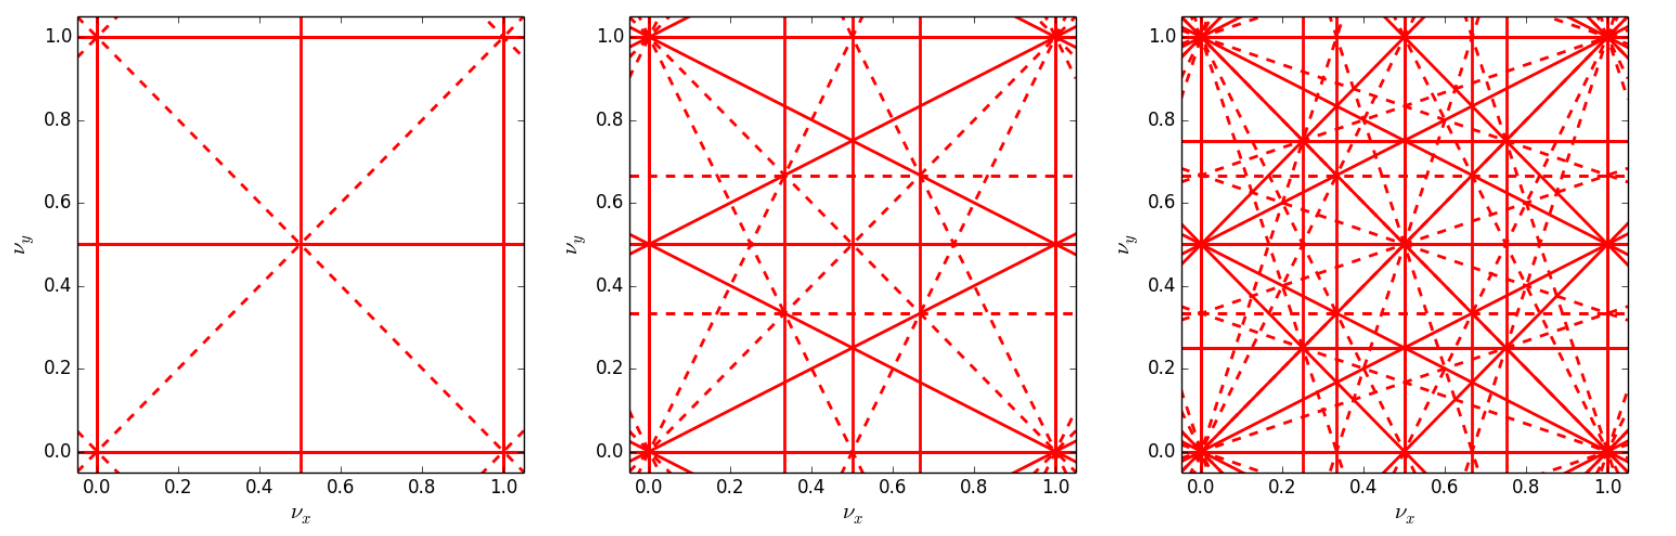
\includegraphics[width=\textwidth]{Images/tunes.png}
    \caption{Resonance lines in tune space up to 2nd, 3rd and 4th order, respectively.}
    \label{resons}
\end{figure}
\subsubsection{Dynamic Aperture}
    Nonlinear dynamics can become sensitive to initial conditions when the amplitudes are large. Because of the tune-shfits, specially the amplitude-dependent tune shifts, the tunes can wander in tune space, eventually crossing resonance conditions that may lead to instabilities, chatotic motion and beam loss. The dynamics can impose limitations to the maximum transverse deviations in which the beam can oscillate while displaying regular and bounded motion. This is a dynamic restriction to the motion known as the \textit{dynamic aperture}.

    Exceeding the dynamic aperture eventually leads to beam loss. During injection of the beam, if the transverse offsets are larger than the dynamic aperture, the beam is not captured into the storage ring. This is specially important for off-axis injection, such as in the case for SIRIUS.

\subsection{Injection scheme for acummulation at SIRIUS storage ring}
Beam acummulation into the storage ring occurs in the off-axis scheme. The beam is delivered at $x\approx-8~\unit{mm}$, and receives the kick from the nonlinear kicker field. The field profile is nonlinear, with zero field and gradient at the center of the axis, so that it does not disturbs the stored beam.
In the off-axis scheme, a sufficiently large dynamic aperture is desired to allow the beam to be captured into the storage ring. The predicted efficiency for SIRIUS setup, considering a dynamic aperture reaching $x=-9~\unit{mm}$, was nearly $100\%$. What was observed during 2022 was an injection efficiency of about $88\pm8\%$.
\lipsum[1-10]

\section{Online Optimization}
This sction describes the experimental methods and analysis employed for optimizing the nonlinear dynamics and evaluating the quality of the configurations found.
\subsection{Dynamic Aperture Optimization}
\subsubsection{Knobs}
The dynamic aperture is determined by the quality of the dynamics in terms of perturbations and nonlinearities. Considering corrected quadrupoles and dipoles (linear optics), the main factors influencing SIRIUS DA are the nonlinearities introduced by the sextupoles and possbibly their field's small errors and deviations from the design parameters. The goal, thus, is to search for the sextupole configurations rendering the largest DA.

The sextupoles are the parmeters which can be tuned, the knobs. SIRIUS has 21 sextupole families: magnets powered by the same power supply. 6 of them are achromatic sextupoles. They are placed where the the dispersion is zero. The 15 other families are chromatic families. Table~\ref{fams} shows the 21 sextupole families names.
 \begin{table}[htb]
    \caption{SIRIUS sextupole families}
    \centering
    \begin{tabular}{cl}
            \hline
            achromatic & \begin{tabular}[c]{@{}l@{}}SFA0, SDA0, \\ SFB0, SDB0,\\ SDP0, SFP0\end{tabular}                                                                \\ \hline
            chromatic  & \begin{tabular}[c]{@{}l@{}}SDA1, SFA1, \\ SDA2, SFA2, \\ SDA3,\\ SDB1, {SFB1}\\ SDB2, SFB2, \\ SDB3, \\ {SFP1}, SDP1,\\ SDP2, SFP2\\ SDP3\end{tabular} \\ \hline
            \end{tabular}
            \label{fams}
            \end{table}
In principle, thus, the optimization parameter space is 21-dimensional. In reality, we would like to change sextupoles without changing chromaticity. Since we need at least one degree of freedom for correcting chromaticity in the horizontal plane and one degree of freedom for correcting the chromaticity in vertical plane, there are 19 available knobs. The dimensionality of the search space can be further reduced by imposing additional constraints to certain families variations. The specific choices of knobs for optimzation experiments are discussed in more details in the Results section.
% In 4th generation Synchrotron storage rings, stronger focusing is needed to deliver lower emittances. Which means stronger sextupole maagnets and more nonlinear dynamics.
\subsubsection{Objective function}
There is no analytical formula for relating the storage ring linear or nonlinear optics to the Dynamic Aperture. The optimization procedure must be a direct search procedure: changes are performed in the knobs and the effect over dynamic aperture is evaluated.

Also, we cannot measure dynamic aperture directly. We must choose an objective function to act as a probe to the DA: a figure of merit related to the dynamic aperture to represent it.

Two objectives usually adopted as probes are the injection efficiency and the beam's resilience to dipolar perturbations. The former is quite self-explanatory: the larger the dynamic aperture, the larger space for the beam to be captured during injection, and thus the larger the injection efficiency. The latter is related to the DA by the following: the larger the horizontal dipolar kicks the beam can survive, the larger the orbit distortions towards the positive or negative horizontal plane (depending on the kick direction). So the larger the amplitudes the beam explores as it oscillates, probing the DA borders. If the beam survives to large kicks, it means the ring can accomodate larger orbit distortions because of an increased dynamic aperture.

In summary, the dynamic aperture optimization procedure must consist on the exploration of sextupole (knobs) configurations yielding the largest dynamic aperture as accessed by as objective function such as injection efficiency or beam kick-resiliency.
\subsubsection{Noise-Robust Online Optimization}
In the optimization literature, optimization routines and algorithms are usually classified according to whether they rely on the calculation of derivatives (gradient-based) or solely on the comparison of the objective function values (gradient-free). The latter can yet be classified into direct- or indirect-search methods, depending on whether the search of the extremum relies on direct comparisons from data or from a mathematical model, respectively \cite{numerical_recipes}.

Both gradient-based and gradient-free strategies rely on the comparison of the objective function at different points of the parameter space. If the objective function suffers from noise this can significantly reduce the efficiency of the optimization routine \cite{numerical_recipes, huang2019beam}. In Chap. 7 of Ref.~\cite{huang2019beam}, a review of the most popular optimization algorithms shows how most of them suffer to find minima to, at least, the precision of the noise-$\sigma$ the objective function is subjected to.

The Robust Conjugate Direction Search (RCDS) algorithm is a indirect-search, gradient-free optimization algorithm introduced in Ref.~\cite{Huang:2013}. The algorithm consists of a main loop for constructing and managing optimal search directions along the knobs space (Powell's Method) and a one-dimensional optimizer responsible for a noise-aware search for the minimum along a given direction. The algorithm is capable of optimizing the objective function (find its local maximum/minimum) to at least the precision of the objective-function noise \cite{Huang:2013, huang2019beam}, being thus adequate for online optimization problems. Specifically, for accelerator controls and optimization, the algorithm has been successfully applied to optimize beam steering and optics matching during injection \cite{Huang:2013}, reducing horizontal emittance \cite{Huang:2013, Huang:2015}and optimization of dynamic aperture \cite{Huang:2013,Huang:2015,Liuzzo:IPAC2016-THPMR015,Olsson:IPAC2018-WEPAL047,yang:ipac2022-tupopt064}.
\subsection{Characterization of Sextupole Magnets Configurations}
Once a configuration of sextupoles (position in parameter space) is found, the nonlinear optics it provides the machine needs to be characterized. The characterizations consisted on evaluatig/measuring the followint figures of merit and desired features
\begin{itemize}
    \item Injection efficiency in nominal off-axis conditions : this is the most desired characteristic. The sextupoles are to be optimized so the DA and the off-axis injection efficiency increase.
    \item Beam Kick resilience: a small current of $2~\unit{\milli\ampere}$, concentrated in a single bucket is stored in the ring. The beam is kicked by the horizontal dipole kicker, which instantly provides a dipolar perturbation leading the beam to be displaced in the horizontal direction. The current before and after the kick is recorded by a current monitor (DCCT) and allows for the calculation of the fraction of the beam lost as a consequence of the kick and the transverse displacement. The procedure is repeated with progressively stronger kicks, and a curve of beam loss as a function of the kick can be constructed. The smaller the losses for larger kicks, the larger the resilience.
    \item Phase portrait area: it is expected that the optimzation procedure increases the dynamic aperture of the machine, meaning it can accomodate larger oscillations and larger phase portraits $x-x^\prime$. Using beam position monitors (BPMs) at the two ends of a straight section, which record the positions of the beam centroid at each turn, we can calculate the position and angle of the beam in the middle of the straight section, and thus recostruct the phase-portrait from turn-by-turn (TbT) data.
    \item Beam lifetime: the lifetime at SIRIUS is dominated by losses due to electron-electron interactions leading to momentum transfers exceeding the energy/momentum acceptance (MA). Optimization of DA does not necessarily leads to improvements in the MA. If the MA is reduced, the rate at which the beam is lost can increase, reducing the total lifetime. It is desireble that the configurations found during DA otpimzation do not worsen the MA and beam lifetime considerably.
    % One dominat effect leading to beam loss is the so-called Touschek Effect, consisiting on collisions between electrons of the same bunch leading to momentum trasfers from the transverse to the longitudinal direction that can exceed the lattice tolerance to momentum deviations, the Momentum Acceptance. Momentum acceptance is the dynamic aperture for off-energy particles. Optimization of DA, which is accesed by the aforementioned objective functions, not necessarily leads to improvements in the MA. If the MA is reduced, the rate of Touschek events increases and thus the lifetime is reduced. Therefore, another desired feature from a good sextupole configurations is having a good beam lifetime. We expect not the worsen the lifetime.
    \item Chromaticity: Sextupoles are introduced in the storage ring for correction of focusing chromatic aberretions. When changing the sextupole settings, it is desired to do so in such a manner that the chromaticity is unchanged. The methods for choosing the optimization knobs already take into account the need for keeping constant chromaticity. Still, after optimization is performed, we need to check whether chromaticity is unchanged.
\end{itemize}
The first two characterizations are quite similar to the two most immediate objective function candidates mentioned above. Indeed, in most nonlinear dynamics optimzation experiments, optimization using injection efficiency or kick resilience as objectives seemed to be completely interchangable. Improvements in injection efficiency necessarily led to improvements in kick resilience, and vice-versa. As shown in more details in the results section, for the SIRIUS storage ring this appears not to be the case. The configurations can be specialized to improvements solely on injection efficiency or solely to kick resilience. This feature was observed during the characterization of the optimized sextupole settings with respect to these two figures of merit.
